\section{Our Approach}
\label{sec:approach}

In this section, we present a approach framework for generating the graph. At the high level, our proposed framework consists of two stage.
\begin{itemize}
    \item {\bf Degree distribution generation.} First, given a certain motif distribution, we train a gradient boosting model using the motif distribution. And then we predict the degree distribution from motif distribution.
    \item {\bf Candidate graph generation.} Second, with the degree distribution, we generate a random graph based on degree distribution as candidate graph for our problem.
    \item {\bf Graph refinement.} Second, the random graph is fed to a heuristic model to refine the graph. The model incorporates the several strategies to refine the graph satisfied the given motif distribution.
\end{itemize}

\subsection{Degree distribution generation} 

In order to better generate random graphs, we assume that all the graphs generated are based on power law degree distributions. The basic idea is to use the motif distribution as features to predict the degree distribution. In this paper, we use Gradient Boosted Regression Trees (GBRT)~\cite{friedman2002stochastic} as the main regression model. Gradient Boosted Regression Trees is a useful machine learning method for regression problems, which also is an ensemble method with combines multiple weak prediction models. It constructs the model in a stage-wise fashion and generalizes the model by optimizing a arbitrary differentiable loss function which in our case is the square loss function\footnote{Square Loss: $\mathcal{L} = (f(x) - y)^2$, here we use $\mathcal{L}$ to describe the squared loss term, $y$ represents the label and $f(x)$ represents the predict score.}. 

More precisely, GBRT trains several small tree regression models (the depth of each tree is 5), each with high bias. Instead of using a uniform weight for each model to prevent the overfitting, GBRT focuses on adding new trees to minimize the current remaining regression error at each iteration. Let $f(x_i)$ denote the prediction score of sample $x_i$ and $\mathcal{L}(f(x_1),...,f(x_n))$ as the loss function of the model, which reaches a minimum if $f(x_i) = y_i$ for all $x_i$. For each new tree $T_i$, that is added into the existing classifier and the current prediction $P(x_i)$, we use the following step:
$$P(x_i) \leftarrow P(x_i) + \alpha \frac{\mathcal{L}}{P(x_i)}$$
\noindent where $\alpha$ is the learning rate, and the gradient $\frac{\mathcal{L}}{P(x_i)}$ is approximated with the prediction score of regression tree~\cite{zheng2007general}. Algorithm~\ref{algo:gbrt} shows the details of GBRT.

\begin{algorithm}
\caption{Gradient Boosted Regression Trees (GBRT). DT indicates the decision tree model which has three parameters, data $D$, #features\mbox{ }f and the depth $d$ of tree.}\label{algo:gbrt}
\begin{algorithmic}
\State \textbf{Input:} Data set $\mathcal{D} =\{(x_1, y_1),..., (x_n, y_n)\}$, learning rate\mbox{ }\alpha, \#Trees\mbox{ }$M$, depth\mbox{ }$d$ \\
\State \textbf{Output:} Combined tree model T

\State Initialization: $\forall i, p_i \leftarrow y_i$

\For {$i = 1$ to $M$} {
    $T_i \leftarrow DT(\{(x_1, p_1),..., (x_n, p_n)\}, f, d)$ \\
    \For {$j = 1$ to $n$} {
        $p_i \leftarrow p_i - \alpha T_i(x_i)$\\
    }
}
$T \leftarrow \alpha \sum_{i = 1}^M T_i$\\
\Return T\\
\end{algorithmic}
\end{algorithm}

\vpara{Implement Note.} In the Decision Tree model, we train $M = 1000$ trees and for each tree tree random select $f = \#\mbox{features} / 10$ and set the depth to 5. If $M$ is too big, the algorithm starts overfitting. As for learning rate, we use $\alpha = 0.001$.


\hide{We use the motif distribution to predict the degree distribution.
For a given motif distribution, we use the motif distribution to predict degree distribution. The idea of this problem is using the motif distribution as a feature to train a model, and then predict a degree distribution for the given motif distribution. More precisely, we use gradient boosting as the main regression method to train a model. Gradient Boosting Tree~\cite{friedman2002stochastic} is a useful machine learning method for regression problems, which also an ensemble method with combine multiple weak prediction models. It makes the model in a stage-wise fashion and generalizes the model by optimization of the arbitrary differentiable loss function which is same as logistic regression. Here we use the python package build in~\cite{pedregosa2011scikit}. Our approach shows good performance. We achieved less than 1\% on Average Relative Error.
}

\vpara{Evaluation Measures} To quantitatively evaluate the performance of predicting the degree distribution, we conducted experiments with different networks. For each network, we evaluated the approaches in terms of \textbf{Average Relative Error (ARE)}.

\vpara{Prediction Performance} We use 168 different networks as input data to evaluate the proposed model, with 10-fold cross validation. In order to avoid bias, we test the data 10 times, and get the prediction alpha for each network. This model achieves \textbf{Average Relative Error (ARE)} sore $0.005521$ with standard deviation $0.00316$.

\subsection{Candidate graph generation}

According the degree distribution we got at stage 1, we use 


=======================================

In this section, we propose a heuristic method for generating the required
graph.

\subsection{Hill climbing}
Hill-climbing is a standard technique for finding good solutions to optimization problems.  Start with a solution that is not particularly good.  At each step, perturb the solution randomly.  If the new answer is better, keep it; if not, keep the old solution.  Repeat this until the algorithm converges to a good solution.

Hill-climbing does not guarantee an optimal solution, since it tends to get stuck at local maxima.  Yet in practice the solutions it finds are "pretty good," especially after running the algorithm several times and picking the best solution.

In our case we minimize the error between the desired motif counts and our solution's motif counts:
\begin{equation}
\label{eqn:avgRelativeError}
\mbox{Average relative error} = \frac{1}{\ell} \sum_{i = 1}^{\ell} \frac{|\mbox{counts}_i - \widehat{\mbox{counts}}_i| + 1}{|\mbox{counts}_i| + 1}
\end{equation}
where $\ell$ is the number of different motif types.

We use the configuration model to generate a random graph with the required degree sequence.  Then at each step we choose two edges (at random) and swap their endpoints.  We count the motifs and compare the error with the new counts to the error with the old counts.  If the new counts give a smaller error, we keep the new graph; otherwise, we discard it.

\begin{algorithm}[t]
\caption{Naive approach}
\label{algorithm:naive}
\begin{algorithmic}
Initialize graph $G = (V, E)$ with prescribed degree sequence\\
motifCounts <- CountMotifs($G$)\\
\Repeat{computation time limit exceeded} {
	Choose $e_1, e_2 \in E$ at random\\
	Add edges $(e_1.Src, e_2.Dst)$, $(e_2.Src, e_1.Dst)$\\
	Delete edges $(e_1.Src, e_1.Dst)$, $(e_2.Src, e_2.Dst)$\\
	newMotifCounts <- CountMotifs($G$)\\
	\eIf {error(newMotifCounts) < error(motifCounts)} {
		motifCounts <- newMotifCounts\\
	} {
		Return graph to original state\\
	}
}

\end{algorithmic}
\end{algorithm}

\subsection{Optimizations}
As written, this solution is very slow.  Counting motifs is $O(|V|^4)$ and takes unacceptably long in practice.  To get good results in practice, we need a large number of rewiring steps, so ideally each rewiring step should take less than a second.

We can speed this up by counting motifs incrementally.  Instead of considering the whole graph on every step, we only look at the part of the graph whose motifs would be affected by the edge changes.  Since we are only looking at motifs with fewer than $5$ nodes, we can only consider the nodes that are one or two hops away from the nodes whose edges are being rewired.  Then we can count how many motifs are being created or destroyed in the induced subgraph on those nodes, and add those to the total motif counts.  Once we have the induced subgraph, we count the motifs by taking all possible sets of four vertices, and seeing which motif they form, if any.

(In our algorithm we break the rewiring step into four steps, two edge deletions and two edge creations.  This way we only measure the effect of one edge creation/deletion step at a time.)

This is still fairly slow, so we apply one final optimization.  We notice that for a 4-motif to be affected by the edge changes, vertices $1$ and $2$ of the motif must be endpoints of the edge.  Vertex $3$ must be an immediate neighbor of an endpoint, and vertex $4$ is either an immediate neighbor or a second-degree neighbor.  Ordinarily, we would have to loop through the immediate neighbors to find all possibilities for vertex $3$, and perform an inner loop through the second degree neighbors to find all possibilities for vertex $4$.  But if vertex $4$ was always an immediate neighbor, we could loop through the immediate neighbors both times, which would speed up the algorithm considerably.

Vertex $4$ is not always an immediate neighbor of vertex $1$ or vertex $2$.  However, when it's not an immediate neighbor of either endpoint, we can do a lot less computation than we would have to otherwise.  We can break these situations up into three cases:

\begin{figure}[t]
\centering
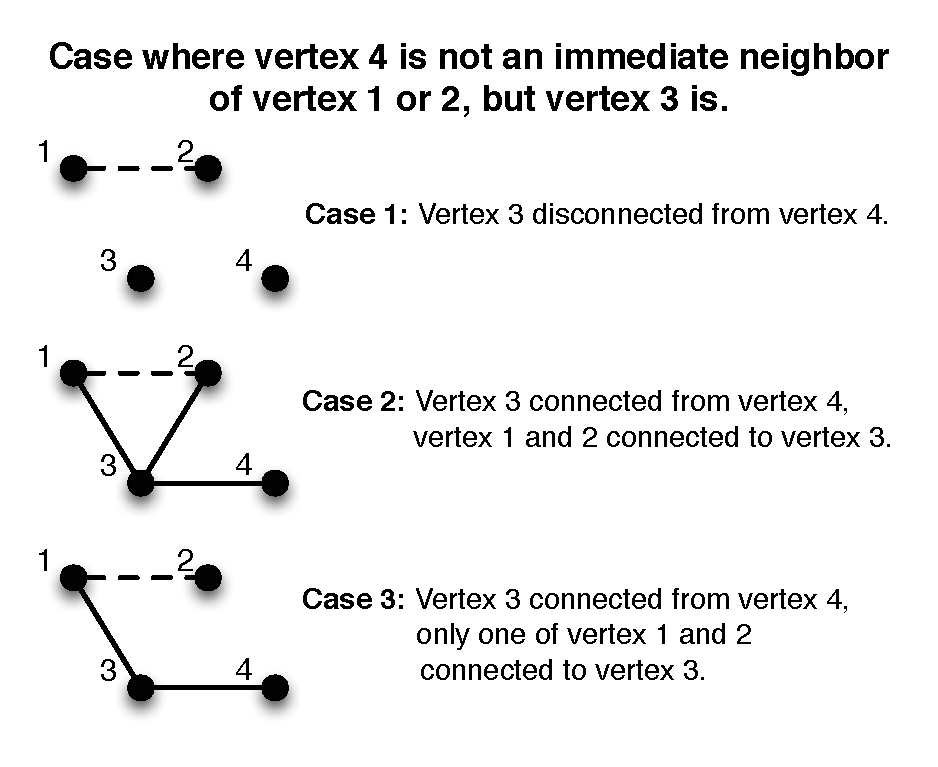
\includegraphics[width=3in]{Figures/case1.eps}
\label{fig:case}
\end{figure}

\begin{itemize}
\item Vertex $3$ is not connected to vertex $4$.  In this case, the four vertices can never form a 4-motif, regardless of whether vertices $1$ and $2$ are connected, and we don't have to change the motif counts.
\item Vertex $3$ and $4$ are connected, and vertex $1$ and $2$ are both connected to vertex $3$.  In this case, connecting vertex $1$ and $2$ deletes a four-star motif and adds a triangle-with-edge motif.
\item Vertex $3$ and $4$ are connected, and only one of vertex $1$ and $2$ are connected to vertex $3$.  In this case, connecting vertex $1$ and $2$ creates a four-line motif.
\end{itemize}

It is much faster to test for these cases than to do the normal
computations (which would involve finding the induced subgraph on those
four vertices, then testing it to see if it was either of the 4-motifs).
So implementing this optimization produces an enormous speedup, allowing us
to perform several thousand rewiring steps in one day.  Each rewiring step
is $O((d_1 + d_2)^2)$, where $d_1$ is the degree of vertex $v_1$, $d_2$
is the degree of vertex $v_2$, and $d_1 + d_2$ is an upper bound on the 
number of first-degree neighbors of $v_1$ and $v_2$.

\subsection{Random restarts}

Hill climbing is an imperfect solution since it is easy to get stuck at
local minima.  We fix this with the method of random restarts.  When we
reach a local minimum, we save the graph and begin rewiring edges randomly.
After this we run hill climbing until we reach another local minimum, then 
repeat the process.  At the end of the computation we return the graph with
lowest error.

We assume the algorithm has reached a local minimum if we have gone through
$|E|$ consecutive rewiring steps without changing the graph.  At this
point, we rewire $|E|/8$ edge pairs randomly and proceed with hill
climbing.  Preliminary results for this approach are presented in 
Section~\ref{sec:exp}.
